\documentclass[12pt,a4paper]{article}

\usepackage[utf8]{inputenc}
\usepackage[T1]{fontenc}
\usepackage[brazil]{babel}
\usepackage{geometry}
\usepackage{multicol}
\usepackage{amsthm}
\usepackage{amssymb}
\usepackage{amsfonts}
\usepackage{mathtools}
\usepackage{xcolor}
\usepackage{enumitem}
\usepackage{tikz}
\usepackage{fancyvrb}
\usepackage[framemethod=tikz]{mdframed}
\usepackage{xspace}
\usepackage{xifthen}
\usepackage{listings}
\usepackage{pdfpages}
\usepackage{titlesec}
\usepackage{graphicx}
\usepackage[hidelinks]{hyperref}
\usepackage[portuguese,onelanguage,linesnumbered,noline,noend]{algorithm2e}

% load times font
\usepackage{mathptmx}
\usepackage[scaled=.90]{helvet}
\usepackage{courier}
\DeclareMathAlphabet{\mathcal}{OMS}{cmsy}{m}{n} % uses default mathcal font

% estilo
\sloppy
\geometry{left=2.5cm,right=2cm,top=2cm,bottom=2.5cm}

\DeclareTextFontCommand{\emph}{\em\color{coralerta}}
\newcommand{\alert}[1]{{\color{coralerta}#1}}

% cores
\colorlet{coralerta}{red!60}
\colorlet{cordefs}{blue!70}

% algoritmos
\newcommand{\textonormal}[1]{#1}
\SetFuncArgSty{textonormal}
\SetProgSty{textonormal}
\SetArgSty{textonormal}

\DontPrintSemicolon
\makeatletter
\newcommand{\Algoritmo}[1]{{\color{coralerta}
    \algocf@seteveryparnl{\relax}
    \hspace*{-2ex}#1:\;
}}
\makeatother

\newcommand{\mysty}[1]{\textbf{\color{black!50}\relsize{-2} #1}}
\SetNlSty{mysty}{}{}

% seções
\titleformat*{\section}{\normalfont\sffamily\large\bfseries\color{cordefs}}
\titleformat*{\subsection}{\bfseries\sffamily\color{cordefs}}
\titleformat*{\subsubsection}{\itshape\subsubsectionfont\color{cordefs}}
\titleformat{\paragraph}{\normalfont\color{cordefs}\bfseries}{}{1em}{}

% teoremas
\mdfdefinestyle{mdteostyle}{
  outerlinewidth = 1pt,
  roundcorner =2pt,
  leftmargin = 0,
  rightmargin = 0,
  backgroundcolor = yellow!10,
  outerlinecolor=blue!10!black,
  innertopmargin = \topskip,
  splittopskip = \topskip,
  ntheorem = true,
  nobreak
}
\newtheoremstyle{coloredthm}
  {0pt}% Space above
  {0pt}% Space below
  {\itshape}% Body font
  {}% Indent amount
  {\bfseries\color{cordefs}}% Theorem head font
  {.}% Punctuation after theorem head
  {.5em}% Space after theorem head
  {}% Theorem head spec (can be left empty, meaning ‘normal’)

\newtheoremstyle{coloredthmnonum}
  {0pt}% Space above
  {0pt}% Space below
  {\itshape}% Body font
  {}% Indent amount
  {\bfseries\color{cordefs}}% Theorem head font
  {.}% Punctuation after theorem head
  {.5em}% Space after theorem head
  {\thmname{#1}\thmnote{ (#3)}}% Theorem head spec (can be left empty, meaning ‘normal’)

\newtheoremstyle{coloredprob}
  {0pt}% Space above
  {0pt}% Space below
  {}% Body font
  {}% Indent amount
  {\bfseries\color{cordefs}}% Theorem head font
  {}% Punctuation after theorem head
  {\newline}% Space after theorem head
  {\thmname{#1}\thmnumber{ #2}\thmnote{: {\color{coralerta}#3}}}% Theorem head spec (can be left empty, meaning ‘normal’)

\theoremstyle{coloredthm}
\newmdtheoremenv[style=mdteostyle]{teorema}{Teorema}
\newmdtheoremenv[style=mdteostyle]{corolario}{Corolário}
\newmdtheoremenv[style=mdteostyle]{fato}{Fato}
\newmdtheoremenv[style=mdteostyle]{lema}{Lema}
\newmdtheoremenv[style=mdteostyle]{afirmacao}{Afirmação}
\newmdtheoremenv[style=mdteostyle]{conjectura}{Conjectura}

\theoremstyle{coloredthmnonum}
\newmdtheoremenv[style=mdteostyle]{definicao}{Definição}

\theoremstyle{coloredprob}
\newmdtheoremenv[style=mdteostyle]{auxproblema}{Problema}

% corrige problema com espaçamento quando teorema e prova começa com lista
\newenvironment{problema}[1][]
  {\begin{auxproblema}[#1]\leavevmode\vspace{-\baselineskip}}
  {\end{auxproblema}}

\renewenvironment{proof}[1][Demonstração]{%
  \def\endqedsymbol{\hfill~\qedsymbol}%
  \renewcommand{\qedhere}{\endqedsymbol\gdef\endqedsymbol{\relax}}%
  \noindent\textit{\color{cordefs}#1.}~}{\endqedsymbol}

% nova lista de questões
\newlist{questions}{enumerate}{2}
\setlist[questions,1]{label={\textbf{Questão \arabic*.}},ref=\arabic*,leftmargin=0pt,align=left,itemindent=*}
\setlist[questions,2]{label={\textbf{\textit{(\alph*)}}},itemsep=0pt}
\newlist{cequestions}{enumerate}{1}
\setlist[cequestions]{label={\textbf{\textit{(\alph*)}}\makebox[0pt][l]{\quad C\quad E \quad}},itemsep=0pt,labelsep=1.7cm,leftmargin=!}

% uso: \resposta[texto]{tamanho}
\newcommand{\resposta}[2][Resposta:]{%
  \par\noindent\ifthenelse{\isempty{#1}}{}{{\small #1\\}}%
  \framebox[\linewidth][l]{\rule{0cm}{#2}}\vspace{1pt}}

\newcommand{\videverso}{\vfill\par\hfill{\emph{\footnotesize(vide verso)}}\clearpage}

\newcommand{\Cabecalho}[1]{
  \thispagestyle{empty}
  \begin{center}\small
    Instituto de Computação -- UNICAMP\\
    Algoritmos de Aproximação\\
    \url{http://www.ic.unicamp.br/~lehilton/mo418a/}\\[10pt]
    {\Large\sffamily\color{cordefs} #1}
\end{center}}

\newcommand{\AutoresData}[2]{{\sf\noindent{\color{cordefs}\textbf{Escrito por:}} #1}\hfill{\sf{\color{cordefs}\textbf{Data:}} #2}}

% \CabecalhoLista{nome da lista}{url random}
\newcommand{\ItensInstrucoes}[1][]{

  \raggedright

  \item Os exercícios devem ser submetidos em formato PDF dentro do prazo
    indicado na página \url{https://www.ic.unicamp.br/~lehilton/mo418a/submit/}.\\
    Utilizem a mesma senha passada em sala para as notas de aula.

  \item Os exercícios devem \emph{escritos à mão} e escaneados. Se for
    fotografar, utilize um aplicativo que corrija a perspectiva. Certifique-se
    de que o documento está legível. Faça um rascunho e passe a limpo.

  \ifx\relax#1\relax\else

  \item Só serão aceitas listas com todas questões respondidas, mas serão
    corrigidos \textbf{apenas} os itens sorteados em \url{#1}.

  \fi
}

% listas
\setlist[itemize,1]{label=$\rightarrow$}
\setlist[itemize,2]{label=--}
\setlist[description]{leftmargin=!,labelwidth=1.8cm}

% configura listing e corrige leitura de centos
\lstset{
  showstringspaces=false,
  basicstyle=\ttfamily,
  inputencoding=utf8,
  extendedchars=true,
  literate={á}{{\'a}}1
    {ã}{{\~a}}1
    {â}{{\^a}}1
    {é}{{\'e}}1
    {ê}{{\^e}}1
    {í}{{\'i}}1
    {ó}{{\'o}}1
    {õ}{{\~o}}1
    {ô}{{\^o}}1
    {ú}{{\'u}}1
    {ç}{{\c c}}1
    {vé}{{v\'e}}2,
}

% % USE:
% %      Teclas     Caractere
% %      AlgGr-Z    «
% %      AltGr-X    »
% %      AltGr-4    £
% \begin{Verbatim}[frame=single,commandchars=£«»]
% // exemplo de código
% int misterio(int a, int b) {
%     if (a < b)
%         return 0;
%     else
%         £textbf«ASD» + misterio(a - b, b);
% }
% \end{Verbatim}

% macros de algoritmos
\newcommand{\ptas}{\ensuremath{\mathrm{PTAS}}\xspace}
\newcommand{\pp}{\ensuremath{\mathrm{P}}\xspace}
\newcommand{\np}{\ensuremath{\mathrm{NP}}\xspace}
\newcommand{\maxsnp}{\ensuremath{\mathrm{MAXSNP}}\xspace}

\newcommand{\val}{\text{val}\xspace}
\newcommand{\opt}{\text{opt}\xspace}
\newcommand{\agm}{\text{agm}\xspace}


\newcommand{\zpli}{\ensuremath{z_{\text{\tiny PLI}}}}
\newcommand{\zpl}{\ensuremath{z_{\text{\tiny PL}}}}

\begin{document}

\Cabecalho{Unique Games Conjecture}

\AutoresData{Felipe L. De Mello, Victor F. Ferrari e Vinícius C. Espindola}{14/11/2019}

\section{Introdução}
\begin{itemize}
    \item Vimos anteriormente um algoritmo de aproximação para o problema Max-Cut.
    \begin{itemize}
        \item Utilizava Semidefinite Programming
        \item .878-aproximação, chamada de algoritmo de \emph{Goemans-Williamson}
    \end{itemize}
    \item Ao final da aula, foi visto um teorema: esse algoritmo é a melhor aproximação possível para o problema, assumindo a \emph{Unique Games Conjecture}.
    \item O que é a Unique Games Conjecture?
\end{itemize}

\subsection{Histórico}
Um aluno de pós-graduação chamado Subhash Khot ficou curioso para saber uma propriedade do problema de coloração em grafos. Já era sabido que decidir se um grafo é 3-colorível é NP-Difícil, mas a dúvida era se aumentar o número de cores disponíveis facilita o problema. Ou seja, se é mais fácil o problema de decidir se necessita de 3 cores, ou K, para qualquer constante K.

A partir desse problema, chegou à conclusão de que deveria estudar a complexidade do problema Unique Games, o que faz sentido ao olhar sua representação em grafo. Assim, em 2002, foi proposta a \emph{Unique Games Conjecture}. História completa pode ser vista em \cite{history}.

\section{Unique Games e Unique Label Cover}

\subsection{Unique Games}
\begin{itemize}
    \item A \textbf{conjectura} do Unique Games é criada a partir do \textbf{problema} chamado Unique Games.
    \item O Unique Games é um problema de satisfação de restrições, ou seja, é uma versão específica do CSP (Constraint Satisfaction Problem).
\end{itemize}

\begin{itemize}
    \item O CSP é dado por:
    \begin{itemize}
        \item Entrada:
            \begin{itemize}
                \item Universo $U$ de valores;
                \item Variáveis $X_i \in U, \forall i \in \{1 \dots n\}$;
                \item restrições $f:U^k \xrightarrow{} \{0,1\}$
            \end{itemize}
        \item Solução: Atribuição de um valor em $U$ para cada variável.
        \item Objetivo: maximizar o número de restrições satisfeitas.
    \end{itemize}
    \item Há a versão com pesos também.
    \item Exemplos de problemas CSP: MAX-CUT, MAX-SAT.
\end{itemize}

\begin{itemize}
    \item O Unique Games é um CSP \emph{binário}, ou seja, cada restrição corresponde a uma função em \emph{duas variáveis}.
    \item Além disso, para cada valor de $U$ de uma das variáveis da restrição, há \emph{exatamente um} valor para a outra variável que a satisfaz. Assim, uma restrição corresponde a uma função \emph{bijetora}.
\end{itemize}

\begin{conjectura}[Unique Games Conjecture: UGC]
    Dados quaisquer $\epsilon,\delta>0$, existe algum $k>0$ dependente de  $\epsilon$ e $\delta$, tal que para o problema Unique Games com universo de tamanho $k$, é \emph{\np-Difícil} distinguir entre instâncias nas quais pelo menos uma fração de $1-\epsilon$ das restrições pode ser satisfeita, e instâncias nas quais no máximo uma fração de $\delta$ das restrições pode ser satisfeita.
\end{conjectura}

\begin{itemize}
    \item Informalmente, a UGC diz que é \np-Difícil diferenciar uma instância do problema na qual \emph{quase todas} as restrições são satisfeitas e uma em que \emph{quase nenhuma} é satisfeita.
    \item Um problema é chamado \emph{UG-Difícil} se ele é \np-Difícil considerando a UGC.
    \item Não se sabe se há algoritmo de aproximação para o Unique Games que garanta desempenho que refute a UGC.
\end{itemize}

\subsection{Unique Label Cover}

\begin{itemize}
    \item Como as restrições do Unique Games são funções de duas variáveis, é fácil perceber que há uma representação do problema como \emph{grafo}.
    \item A versão em grafo do problema possui um nome: \emph{Unique Label Cover}.
    \item Essa versão é tão comum, e mais fácil de entender, que em muitos lugares o Unique Games é apresentado diretamente com ela!
    \item Para a transformação do UG para o ULC, criamos \emph{permutações}.
    \begin{itemize}
        \item Uma permutação é um rearranjo do universo $U$ do problema que mapeia, para cada restrição, o valor de uma variável ao valor da outra tal que $f(X_i,X_j) = 1$.
        \item Isso pode ser feito pois a função é bijetora, e para universo de tamanho $k$, $U={1\dots k}$.
        \item Assim, podemos definir a permutação como $\pi(i) = j$ se $f(i,j) = 1$.
    \end{itemize}
\end{itemize}

Assim, a transformação é:

\begin{algorithm}
  \Algoritmo{Transformação-UG-ULC}
  Crie um grafo vazio não-direcionado $G=(V,E)$\;
  Para cada variável $X_u, u \in {1\dots n}$, insira o vértice $u$ em $V$\;
  Para cada restrição $f(X_u,X_v)$, insira a aresta $(u,v)$ em E\;
  Para toda aresta $(u,v)$, crie uma permutação $\pi_{uv}: U \xrightarrow{} U$ tal que $\pi_{uv}(i)=j$ se $f(i,j)=1$\;
  Retorne $G, \pi$\;
\end{algorithm}

\begin{itemize}
    \item Assim, o problema se torna um de encontrar \emph{labels (rótulos)} em vértices tais que a maior quantidade de permutações são satisfeitas.
    \item Podemos verificar em tempo polinomial se \emph{todas} as arestas do grafo são satisfatíveis.
    \begin{itemize}
        \item Para toda componente conexa do grafo, teste todos os \textit{labels} para um vértice arbitrário.
        \item Para cada escolha, \emph{propague} para todos os outros, pelas permutações.
        \item Se todas as arestas são satisfatíveis, há algum \textit{label} que gera uma atribuição perfeita, e isso pode ser verificado em tempo polinomial, no pior caso.
    \end{itemize}
    \item Similarmente, saber se \emph{nenhuma} aresta é satisfatível também é trivial.
    \item Porém, o mesmo não pode ser dito para todos os outros casos.
    \item Pela UGC, se é desejado saber se uma \textbf{fração constante} de arestas é satisfatível, o problema é \np-Difícil para algum universo, independentemente da fração.
    \item Existe um algoritmo de aproximação de fator $1-\sqrt{\epsilon \log n}$ para o Unique Games/Unique Label Cover, baseado em \emph{Semidefinite Programming}. 
    \begin{itemize}
        \item Esse algoritmo funciona para instâncias nas quais uma fração de $1-\epsilon$ das arestas/restrições são satisfatíveis.
        \item Se $\epsilon \in O(1/\log n)$, essa aproximação é constante.
        \item Não iremos mostrar esse algoritmo hoje, mas está especificado e demonstrado em \cite{design_approx_algs}.
    \end{itemize}
    \item Há também algoritmos \emph{subexponenciais} para o problema e outros relacionados, ao contrário de diversos outros problemas \np-Difíceis. Alguns podem ser vistos em \cite{subexponential}.
\end{itemize}

\section{Consequências da UGC}
\begin{itemize}
    \item Desde 2002, a UGC teve diversas aplicações em problemas relacionados, como pode ser visto na figura \ref{fig:reducoes}.
    \item A figura \ref{fig:reducoes} foi extraída de \cite{survey}, que também possui diversos desenvolvimentos e conclusões em cima da UGC.
    \item Como visto na figura, o principal uso da UGC foi para provas de \emph{inaproximabilidade}, muitas vezes junto com outra técnica, como PCP.
    \item Ela também deu origem a diversas \emph{variantes}.
    \item Deste ponto em diante, veremos duas reduções para problemas que provam inaproximabilidade ou que uma aproximação conhecida é a melhor possível.
\end{itemize}

\begin{figure}
    \centering
    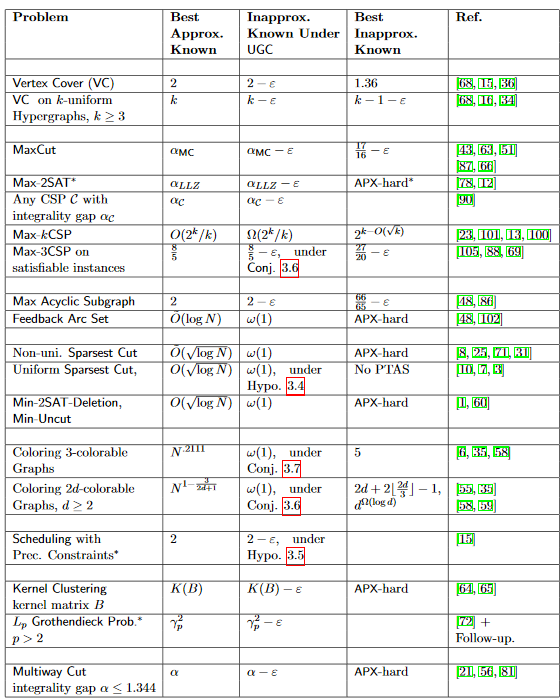
\includegraphics[width=0.8\textwidth]{reducoes.png}
    \caption{Reduções obtidas a partir da UGC.}
    \label{fig:reducoes}
\end{figure}

\section{Redução para Multicut}

\begin{itemize}
    \item Relembrando o problema do multicorte:
        \begin{itemize}
            \item Entrada:
                \begin{itemize}
                    \item grafo G=(V,E);
                    \item custo das arestas $c_e \ge 0,\, e \in E$;
                    \item pares de vértices fonte-ralo $s_1-t_1, \dots, s_k-t_k,\,s,t \in V$.
                \end{itemize}
            \item Solução: conjunto de arestas $F$.
            \item Objetivo: minimizar o número de arestas $|\,F\,|$ nas quais ao serem removidas desconectam todos os pares $s_1-t_1, \dots, s_k-t_k$. 
        \end{itemize}
\end{itemize}        

\begin{teorema} \label{multicut}
    Assumindo a conjectura do Unique Games, para qualquer constante $\alpha \ge 1$, não existe $\alpha$-aproximação para o problema do multicorte a não ser que $\pp = \np$.
\end{teorema}
    
\begin{itemize}
    \item Pelo teorema, é \emph{UG-Difícil} aproximar o problema do multicorte por qualquer constante maior ou igual a 1.
    
    \item Para a redução da UG para multicorte utilizamos um caso especial da UG chamada MAX 2LIN(k).
    
    \item MAX 2LIN(k):
        \begin{itemize}
            \item Entrada:
            \begin{itemize}
                \item L={0,...,k-1}, $k \in \mathbb{Z}$;
                \item Variáveis (vértices) $\in V$;
                \item Restrições (arestas) $\in E$;
                \item $\forall uv \in E$, temos $c_{uv} \in L$ tal que $\pi_{uv}(i)=i-c_{uv}(mod\,k)$, ou seja, $uv$ é satisfeita $\iff$ os vértices $u$ e $v$ recebem rótulos $i,j$ tais que $i-j=c_{uv}(mod\,k)$;
            \end{itemize}
            \item Solução: Atribuição de rótulos R, tal que  $\forall u \in V$, existe um rótulo $r_u \in L$;
            \item Objetivo: Maximizar número de arestas $uv \in E$ satisfeitas.
        \end{itemize}

\begin{conjectura}[Linear Unique Games Conjecture: LUGC]
    Dados quaisquer $\epsilon,\delta>0$, existe algum $k>0$ dependente de  $\epsilon$ e $\delta$, a versão do unique games MAX 2LIN(k) com L={0,...,k-1}, é \emph{\np-Difícil} distinguir entre instâncias nas quais pelo menos uma fração de $1-\epsilon$ das arestas pode ser satisfeita, e instâncias nas quais no máximo uma fração de $\delta$ das arestas pode ser satisfeita.
\end{conjectura}

     \item Para provar o \emph{Teorema \ref{multicut}} são necessários 2 lemas:
    \begin{lema} \label{lema1multicut}
        Para qualquer $\epsilon$ tal que $0 \le \epsilon \le 1$, dado uma solução viável de uma instância de  MAX 2LIN(k) que satisfaz pelo menos $(1-\epsilon)|\,E\,|$ arestas, então existe uma solução viável para uma instância do multicut com custo de no máximo $\epsilon|\,E'\,|$.
    \end{lema}
    \begin{proof}[Prova do Lema \ref{lema1multicut}]
        Reduzir MAX 2LIN(k) para multicorte:
        \begin{itemize}
            \item Seja I uma instância do MAX 2LIN(k) com grafo $G=(V,E)$, universo $L$ de rótulos de tamanho $k$ e $C$ o conjunto de pesos das arestas de $E$;
            \item Faça uma instância I' do multicorte da seguinte maneira: 
            \begin{itemize}
                \item G'=(V',E') com V' = V x L;
                \item Arestas em E' entre pares vértice-rótulo (u,i) e (v,j) $\iff uv \in E$ e $i-j=c_{uv}(mod\,k)$;
                \item Também faça os pares fontes-ralo serem s=(u,i) e t=(u,j) para todo u $\in V$ e $i \ne j$;
            \end{itemize}
            \item Note que $E'=k|\,E\,|$ e $V'=k|\,V\,|$;
            \item Suponha uma rotulação $x_u \in L$ de G que satisfaz pelo menos $(1-\epsilon)|\,E\,|$ arestas de G;
            \item Particione V' em k partes, $V'_0,\dots,V'_{k-1}$, onde $V'_c=\{(u,x_u+c(mod\,k))\} \forall u \in V$, ou seja, a c-ésima parte será o conjunto de vértices cuja rotulação satisfazem uma aresta de custo c;          \item Note que s=(u,i) e t=(u,j) $\forall u\in V$ e $i \ne j$; estão em diferentes partes da partição, portanto, ao remover todas arestas com extremos em diferentes partes da partição obtemos uma solução do multicorte;
            \item Agora determinamos o custo desta solução. Considere qualquer aresta $((u,i),(v,j)) \in E’$ tal que (u,i) e (v,j) estão em diferentes partes da partição. Demonstraremos que a aresta (u,v) no grafo original não é satisfeita pelo rotulamento dado;
            \item Pela construção de E’ sabemos que $i-j=c_{uv}(mod\,k)$. Também sabemos que (u,i) e (v,j) estão em diferentes partes da partição;
            \item Suponha que $(u,i) \in V_c$ e $(v,j) \in V_c$' para $c \ne c'$. Então $i=x_u+c(mod\,k)$ e $j=x_v+c'(mod\,k)$, e portanto:
            \begin{align*}
                c_{uv} &= i-j(mod\,k) \\
                       &= (x_u+c)-(x_v+c')(mod\,k) \\
                       &= (x_u-x_v)+(c+c')(mod\,k) \\
                       &\ne x_u-x_v(mod\,k)
            \end{align*}
            pois $c \ne c'$;
            \item Como uma aresta é satisfeita $\iff c_{uv} = i-j(mod\,k)$, isto significa que arestas entre vértices de diferentes partições não são satisfeitas. Como no máximo $\epsilon|\,E\,|$ arestas não são satisfeitas em MAX 2LIN(k), no máximo $\epsilon k|\,E\,| = \epsilon|\,E'\,|$ arestas são removidas no multicorte.
        \end{itemize}
    \end{proof}
    \begin{lema} \label{lema2multicut}
        Para qualquer $\epsilon$ tal que $0 \le \epsilon \le 1$, dado uma solução de uma instância do multicorte de custo máximo $\epsilon|\,E'\,|$, então existe uma solução para uma instância do MAX 2LIN(k) que satisfaz pelo menos (1-2$\epsilon$)$|\,E\,|$ arestas.
    \end{lema}
    \begin{proof}[Prova do Lema \ref{lema2multicut}] omitida por simplificação, mas é o caminho inverso da prova do Lema \ref{lema1multicut}. Pode ser vista em \cite{design_approx_algs}.
    \end{proof}\\\\
    \begin{proof}[Prova do Teorema \ref{multicut}]
    \begin{itemize}
        \item Suponha que existe $\alpha$-aproximação para o problema do multicorte;
        \item Então utilizando este algoritmo e o Lema \ref{lema1multicut}, sabemos que: dado uma instância do MAX LIN2(k), na qual pelo menos (1-$\epsilon$)$|\,E\,|$ arestas são satisfeitas, podemos encontrar uma solução do multicorte de custo $\epsilon \alpha|\,E'\,|$;
        \item Pelo Lema \ref{lema2multicut} sabemos obter uma solução do MAX 2LIN(k), a partir deste multicorte, na qual pelo menos (1-2$\epsilon \alpha$)$|\,E\,|$ arestas satisfeitas;
        \item Se a instância do MAX LIN2(k) satisfaz no máximo $\delta|\,E\,|$ arestas, então este algoritmo satisfaz no máximo $\delta|\,E\,|$ arestas;
        \item Fazendo $\epsilon < \frac{1-\delta}{2\alpha}$, então temos que $(1-2\epsilon\alpha)|\,E\,| > \delta|\,E\,|$.
        \item Isto implica que nosso algoritmo consegue distinguir entre instâncias nas quais pelo menos (1-$\epsilon$)$|\,E\,|$ arestas são satisfeitas e instâncias nas quais no máximo $\delta|\,E\,|$ arestas são satisfeitas;
        \item Dado a UG, isto implica que $\pp = \np$.
    \end{itemize}
    \end{proof}
\end{itemize}

\section{Redução para Max-Cut}
\begin{itemize}
    \item Relembrando o problema Max-Cut:
    \begin{itemize}
        \item Entrada:
            \begin{itemize}
                \item grafo G=(V,E);
                \item pesos $\omega: E \xrightarrow{} \mathbb{R_+}$
            \end{itemize}
        \item Solução: corte $[S,T], V=S \cup T$.
        \item Objetivo: max $\sum_{(i,j) \in E[S,T]}\omega_{ij}$
        \item $E[S,T]$ são arestas $(i,j)$ com $i \in S$ e $j \in T$.
    \end{itemize}
\end{itemize}    

\begin{teorema} \label{maxcut}
    Assumindo a conjectura do Unique Games, não existe $\alpha$-aproximação para o problema do corte máximo com constante
    \[\alpha > \min_{-1 \le x \le 1} \frac{\frac{1}{\pi} \arccos{x}}{\frac{1}{2}(1-x)} \ge .878 \]
    a não ser que $\pp = \np$.
\end{teorema}

\begin{itemize}
    \item Ou seja, queremos provar que o algoritmo de Goemans-Williamson possui o \emph{melhor fator de aproximação} para o Max-Cut, dada a UGC.
    \item É, então, UG-Difícil aproximar o problema por um fator melhor que .878.
    \item A prova completa é muito complexa, envolve conceitos um pouco mais específicos de \emph{PCP}, então as ideias serão resumidas.
    \item Esse mesmo método é utilizado para provar diversos outros resultados em relação ao UGC.
    \item Para o problema, introduzimos uma nova variante da UGC, para o caso em que os grafos são bipartidos e os graus dos vértices em uma partição são os mesmos.
\end{itemize}

\begin{conjectura}[Bipartite Unique Games Conjecture: BUGC]
    Dados quaisquer $\epsilon,\delta>0$, existe algum $k>0$ dependente de $\epsilon$ e $\delta$, tal que para o problema Unique Games com universo de tamanho $k$ em grafos bipartidos nos quais todos os vértices de uma partição têm o mesmo grau, é \np-Difícil distinguir entre instâncias nas quais pelo menos uma fração de $1-\epsilon$ das restrições pode ser satisfeita, e instâncias nas quais no máximo uma fração de $\delta$ das restrições pode ser satisfeita.
\end{conjectura}

\begin{itemize}
    \item Não provaremos a equivalência entre a BUGC e a UGC, assim como não o fizemos para a LUGC.
    \item A partir dela, podemos enunciar o seguinte teorema, que é o principal resultado para provar o teorema \ref{maxcut}:
\end{itemize}

\begin{teorema}[BUGC-PCP]\label{bugc-pcp}
    Supondo a BUGC, para qualquer constante positiva $\gamma>0$ e qualquer $\rho \in (-1,0)$, $\np \subseteq PCP(\log (n),2)$, onde o verificador tem \textit{completeness} no mínimo $\frac{1}{2} (1-\rho)-\gamma$ e \textit{soundness} no máximo $\frac{1}{\pi} \arccos{\rho} + \gamma$ e o verificador aceita apenas se dois bits não são iguais.
\end{teorema}

\begin{proof}[Prova do Teorema \ref{maxcut}]

\begin{itemize}
    \item Para qualquer instância de um problema \np-Completo $\Pi$ e um verificador como o do Teorema \ref{bugc-pcp}, podemos criar uma instância $G(V_1,V_2,E)$ do Max-Cut equivalente ao CSP gerado:
    \begin{itemize}
        \item Sejam os bits lidos da prova vértices de $G$, de forma que:
            \begin{itemize}
                \item Se $v=0$, então $v \in V_1$
                \item Se $v=1$, então $v \in V_2$
            \end{itemize}
        \item Para toda possível \textit{string} de bits do verificador, cria-se uma aresta $e\in E$, tal que:
            \begin{itemize}
                \item Se vértices comparados tem mesmo valor, então $e$ não entra no corte
                \item Se vértices comparados valores distintos, então $e$ entra no corte
            \end{itemize}
        \item Por construção, o número de restrições satisfeitas no SCP representa o número de arestas no corte do grafo G.
    \end{itemize}
    \item Pelos conceitos de PCP, temos que:
        \begin{itemize}
            \item Instâncias SIM de $\Pi$ terão pelo menos uma fração $c$ de restrições aceitas
            \item Instâncias NÃO de $\Pi$ terão no máximo uma fração $s$ de restrições aceitas
        \end{itemize}
    \item Tais condições implicam que qualquer $\alpha$-aproximação, tal que $\alpha > \frac{s}{c}$, resultariam em distinguir entre instâncias SIM e NÃO do problema $\pi$, \np-Completo, em tempo polinomial.
    \item Como isso é válido para quaisquer $\gamma > 0$ e $\rho \in (-1,0)$, temos que não existe $\alpha$-aproximação para $\alpha > \min_{\rho \in (-1,0)} \frac{s}{c}$.
    \item Enfim, vemos que $\min_{\rho \in (-1,0)} \frac{s}{c} = \min_{\rho \in (-1,1)} \frac{s}{c}= \min_{\rho \in (-1,1)} \frac{\frac{1}{\pi} \arccos{\rho}}{\frac{1}{2}(1-\rho)}$.
    \item Assim, considerando o Teorema \ref{bugc-pcp}, o Teorema \ref{maxcut} é verdade: não há $\alpha$-aproximação para o Max-Cut para $\alpha > .878$, a não ser que $\pp=\np$.
\end{itemize}
\end{proof}

\subsection{Construindo o Verificador PCP}
\begin{itemize}
    \item Precisamos criar um algoritimo verificador de forma que as condições do Teorema \ref{bugc-pcp} sejam satisfeitas.
    \item Criaremos um algoritimo verificador e mostraremos que há uma prova $\pi$ para uma instância SIM do BUGC em que o verificador aceita com probabilidade $\geq completeness = \frac{1}{2}(1-\rho)$
    \item \textcolor{red}{Soundness não será provada.}
    \item \textbf{Conceitos necessários:}
    \begin{itemize}
        \item \textit{\textbf{Funções ditadoras:}} $f:\{0,1\}^k \xrightarrow\ \{0,1\}$, tal que para $f(b_1,b_2,...,b_k)=b_i$ tal que $i\in [0,k]$
        \item \textit{\textbf{Ruído:}} Dado $x\in \{0,1\}^k$, podemos criar $y$ invertendo independentemente cada bit de $x$ com probabilidadade $\frac{1}{2} (1-\rho)$. Denota-se esse processo por $y\sim_\rho x$.
        \item \textit{\textbf{Bits permutados pela aresta:}}  Dado $x\in \{0,1\}^k$ e uma permutação $\pi:[k]\xrightarrow\ [k]$, dada uma aresta $(v,w)$, seja $x \circ \pi_{vw} = (x_{\pi vw(1)},x_{\pi vw(2)},...,x_{\pi vw(k)})$.
        \item \textbf{Observações:}
            \begin{itemize}
                \item A sensibilidade à ruído de uma função ditadora é equivalente a probabilidade de o bit ditador ser invertido
            \end{itemize}
    \end{itemize}
    
    \item Note que dada a aresta $(v,w)$ onde $v$ tem rótulo $i$ codificado por $f_v$ e $w$ tem rótulo $j$ codificado por $f_w$, temos que $f_v(x)=f_w(x\circ \pi_{vw})$ para todo $x\in \{0,1\}^k$.
    \item Queremos codificar uma prova para uma instância SIM do BUGC.\\
    Dada uma rotulação como prova, codificaremos os rótulos de todos os vértices $v$ em bits da seguinte forma:
    \begin{itemize}
        \item Cria-se uma função ditadora $f_v:\{0,1\}^k \xrightarrow\ \{0,1\}$
        \item Para codificar que o vértice $v$ possui rótulo $i$, temos que, para uma entrada $x\in \{0,1\}^k$, $f_v(x)=x_i$ tal que $f_v$ é uma função ditadora e seu resultado é o $i$-ésimo bit de $x$.
        \item Para todas as possíveis \textit{strings} de entrada $x\in \{0,1\}^k$, listamos os possíveis valores de $f_v(x)$ em um bloco de bits.
        \item A prova $\pi$ será a concatenação de todos os blocos de bits gerados para cada um dos vértices codificados da prova.
    \end{itemize}
    
    \item \textbf{Verificador:}
        \begin{itemize}
            \item Dada uma instância $G(V_1,V_2,E)$ do BUG
            \item Seleciona-se $v\in V_1$ aleatoriamente
            \item Seleciona-se dois vizinhos $w,u\in V_2$ de $v$ aleatoriamente e independentemente. \item Seleciona-se uma string aleatória $x\in \{0,1\}^k$ e gera-se $y\sim_\rho x$. 
            \item Por fim, compara os dois bits de prova $f_w(x\circ \pi_{vw})$ e $f_u(y\circ \pi_{vu})$
            \item Retorna SIM se $f_w(x\circ \pi_{vw})\ne f_u(y\circ \pi_{vu})$
        \end{itemize}
    
\subsection{Completeness}
    \begin{lema} \label{completeness}
        Para qualquer $\rho \in [-1,1]$, se pelo menos uma fração de $1-\epsilon$ das arestas da instância do BUG são satisfeitas, então pode-se provar que o verificador aceita a prova com probabilidade de pelo menos $(1-2\epsilon)\cdot \frac{1}{2}(1-\rho)$.
    \end{lema}
    \begin{proof}[Prova do Lema \ref{completeness}]
        \item Probabilidade de que o verificador descrito com a prova $\pi$ e uma instância SIM da BUGC (que tenha pelo menos uma fração $\frac{1}{2}(1-\rho)$ da arestas satisfatíveis) retorna SIM:
        \begin{itemize}
            \item Probabilidade de $(v,w)$ seja satifatível é $\geq (1-\epsilon)$
            \item Probabilidade de $(v,u)$ seja satifatível é $\geq (1-\epsilon)$
            \item Probabilidade de ambas $(v,w)$ e $(v,u)$ serem satisfeitas é $\geq (1-2\epsilon)$
            \item Probabilidade de que $f_w(x\circ \pi_{vw}) = f_u(x\circ \pi_{vu})$ é $\geq (1-2\epsilon)$
            \item Probabilidade de que $f_u(x\circ \pi_{vu})\ne f_u(y\circ \pi_{vu})$ é $\frac{1}{2}(1-\rho)$
            \item Probabilidade de que $f_w(x\circ \pi_{vw}) = f_u(x\circ \pi_{vu})$ e $f_u(x\circ \pi_{vu})\ne f_u(y\circ \pi_{vu})$ é equivalente a probabilidade de que $f_w(x\circ \pi_{vw})\ne f_u(y\circ \pi_{vu})$
            \item Portanto, retorna SIM com probabilidade $\geq (1-2\epsilon)\frac{1}{2}(1-\rho) $ 
        \end{itemize}
        
        \item Provamos a \textit{completeness} do verificador.
    \end{proof}


\subsection{Soundness} 
  
    \begin{lema} \label{soundness}
        Para qualquer $\rho \in (-1, 0)$ e qualquer $\gamma>0$, se pelo menos uma fração $\delta$ das arestas da instância do BUG forem satisfatíveis, então pode-se provar que  o verificador aceita a instância com probabilidade de no máximo $\frac{1}{\pi}\arccos{\rho} + \gamma$
    \end{lema}
    \begin{proof}[Prova do Lema \ref{soundness}]
        \item Parte difícil da prova da redução. Não será discutida aqui.
        \item Pode ser encontrada em \cite{maxcut}.
        \item Aceitemos que o \textit{soundness} do Teorema \ref{bugc-pcp} vale:\\
        Para uma instância NÃO do BUGC (ou seja, no máximo uma fração $s\leq \frac{1}{\pi}\arccos\rho$ das arestas são satisfeitas), temos que o verificador retorna SIM para qualquer prova $\pi$ com probabilidade de no máximo $s$. 
    \end{proof}

\subsection{Concluindo}
    
    \item Os Lemas \ref{completeness} e \ref{soundness} provam que podemos criar o verificador PCP do Teorema \ref{bugc-pcp};
    \item Temos que o Teorema \ref{bugc-pcp} implica o Teorema \ref{maxcut}, dada a redução do verificador para o Max-Cut;
    \item \textbf{Concluindo, o Teorema \ref{maxcut} (inaproximabilidade do Max-Cut para $\alpha > .878$) é verdadeiro.}

\end{itemize}
  
\section{2-2 Games Conjecture}
\begin{itemize}
    \item Durante muito tempo, a comunidade acadêmica ficou dividida no que tange à veracidade da UGC. Ainda assim, é tópico de pesquisa há muitos anos, assim como suas variantes.
    \item Uma variação do Unique Games é o \emph{2-2 Games}. Nesse problema, em vez das \textit{labels} serem únicas para uma restrição, existem \emph{duas alternativas} que a satisfazem.
    \item Em janeiro de 2018, um artigo foi publicado pelo Subhash Khot (com outros pesquisadores) que, unido com outros publicados recentemente, \emph{prova} a 2-2 Games Conjecture, variante mais fraca da UGC para o 2-2 Games.
    \item Isso convenceu muitos céticos (alguns dos maiores céticos!) de que a UGC deve ser verdadeira, pela proximidade em relação ao 2-2 GC.
    \item É dito que isso prova \emph{metade} da UGC.
    \item Mais informações sobre a 2-2 Games Conjecture e suas consequências em \cite{history}.
\end{itemize}

\section*{Exercício}
    \begin{itemize}
        \item a) Dado a instância do problema do Unique Games a seguir, construa uma instância equivalente do problema Unique Label Cover (vértices, arestas e permutações):
    
    Universo: U = \{0, 1, 2, 3\};
    
    Variáveis: $x_a, x_b, x_c, x_d$;
    
    Restrições:
    
    $f_1(x_a,x_b): f_1(0,2) = 1,f_1(1,3) = 1;$
    
    $f_2(x_a,x_c): f_2(0,2) = 1,f_2(1,3) = 1;$
    
    $f_3(x_b,x_c): f_3(0,1) = 1,f_3(2,3) = 1;$
    
    $f_4(x_c,x_d): f_4(0,3) = 1,f_4(1,2) = 1;$
    
    \item b) Verifique se todas as arestas da instância são satisfatíveis.
    
    \item c) Para essa instância pequena, é possível rapidamente verificar quantas arestas são satisfatíveis. Qual a consequência da UGC para o problema, com instâncias quaisquer?
    \end{itemize}

\bibliographystyle{abbrv}
\bibliography{ugc.bib}

\end{document}

